\documentclass [12pt]{article}
\usepackage{amsmath}
\usepackage{amsthm}
\usepackage{amsfonts}
\usepackage{parskip}
\usepackage[margin=1.25in]{geometry}
\usepackage{graphicx}
\usepackage[none]{hyphenat}
\newtheorem*{hypothesis}{Hypothesis}
\newtheorem*{theorem}{Theorem}

\newcommand{\tab}{\hspace{10mm}} 
\graphicspath{ {images/} }

\title{Using Latent Semantic Analysis for Building Literature Recommendation} 
\author{Allen Yu \\ amengyangyu@gmail.com \\ UCLA - Masters of Applied Economics}

\begin{document} 
\maketitle

\begin{abstract}
This paper examines the feasibility of constructing a recommendation system for scientific literature using Latent Semantic Analysis (LSA) with a specific focus on economic literature. A working LSA based recommendation system has been developed. We addressed common data processing issues, system scalability, limitations of the theory, and pragmatic solutions. We find that LSA within a specific field of a discipline results in impressively accurate suggestions, while suggestions for a whole discipline (i.e. economics) only functions well when the actual similarity measure is very high.
\end{abstract}

\section{Introduction} 
With the advent of big data, recommendation and suggestion have become prominent questions to tackle. With all the accrued data on individual persons, how best to improve the user experience? Whether to advertise a product the user is likely to buy or to selectively present media relevant to the user's interest, it is clear that recommendation and suggestion algorithms have an incredible potential to reduce search costs for the user in a variety of different fields. 

Much of the current efforts in this field are geared toward improving user experience. That is, accurate suggestions and recommendations provide value to users to incentivize them to continue using the particular product. However, relatively little effort has been expended in examining how an efficient recommendation system might improve worker productivity in professions where specific information is necessary but difficult to obtain. One such field is academia. Academia is an area with relatively low financial backing and financial incentives compared with other sectors of the economy, and yet academia possesses one of the highest returns of a dollar to the overall wellbeing of the economy. Cost-efficient methods for increasing efficiency for these members of society, could be a relatively easy way to improve overall long-term economic welfare.

Although academic literature databases exists, effective suggestion of articles on particular esoteric topics is rarely achieved by the content providers and is more often the result of word of mouth between fellow academics when sharing ideas. In general, the search cost of relevant information in Academia is very high due to the width and depth of ideas. Not only is the span of ideas in a given field incredibly wide, but the depth of topics is extremely complex. Therefore, the focus of this paper is to examine basic low-level constructions of recommendation systems for academic literature, focusing on the efficacy and pragmatism of implementation. 

\section{Background  -  LSA} 
\subsection{Distributional Semantics}
The main technique that this paper is based off of is Latent Semantic Analysis (LSA). We provide a brief introduction to the process of LSA and its main mathematical method Singular Value Decomposition (SVD). LSA is built upon assumptions from Distributional Semantics, in particular the Distributional Hypothesis. The hypothesis is as follows: 

\ 
\begin{hypothesis}[Distributional Hypothesis]
Ideas on a macroscopic scale are conveyed through a distribution of words. Therefore, linguistic texts with similar distributions of words are semantically similar. Conversely, words that are semantically similar will have similar distributions across texts. 
\end{hypothesis} 

Under this assumption, the main object of LSA is to construct some measure of the frequencies of words across the documents. To this end, the first step of LSA entails the creation of the TD-IDF matrix. 

\subsection{TD-IDF Matrix} 
The TD-IDF matrix is composed of multiplying two parts:

1. TD - Term Document Matrix 

2. IDF - Inverse Document Frequency

The Term Document Matrix is a matrix of frequencies. One dimension represents the set terms selected from the corpus (our body of documents) and the other dimension representing every single document that exists within the corpus. A given entry $(i, j)$ in the matrix is the frequency of term $i$ in document $j$. 

One might raise a question to why the semantic space (dimension of terms) is not of every unique word encountered. This is because many terms are useless in helping determine similarity. Pronouns (e.g. it, he,  she) are  prominent examples. We will discuss the filtering process of adding terms to our semantic space in the Datasets sections. 



\begin{center} 
 
      \textbf{TD Matrix}

\

   $ \bordermatrix{ & &  Document &Space - (d_n) &   \cr
       &  f_{1,1} & \ldots &  \ldots &  f_{1, n} \cr
       &  \vdots& &  &  \vdots \cr
      Semantic&   & \ddots  & &   \cr
       Space - (t_m) & \vdots  &  &    &  \vdots\cr
     &    &   &  \ddots  &  \cr
      & \vdots  &  &    &  \vdots\cr
      &  f_{m,1} & \ldots & \ldots &  f_{m, n}}   \qquad$
     
      
 \end{center}
 
 Where $f_{i, j}$ is the the number of times that term $t_i$ occurs in document $d_j$.
 
 \ 
 
 The Inverse Document Frequency (IDF) is a function that helps scale the TD to account for words that are too common. The IDF is defined as 
 
 $$ idf(t, D) = log\frac{N}{|\{d\in D: t \in d\}|}$$
 
 $D$ is the entire corpus of documents
 
 $N$ is the number of documents, $N = |D|$
 
 $|\{d\in D: t \in d\}|$ describes the number of documents that the term occurs in. 
 
 Notably, when term $t$ is in every single document $d$, the $idf(t, D) = log(1) = 0$. The IDF provides a relative measure to remove ubiquitous terms within a given corpus. Not only does it prevent common terms like `is' or `a' from providing similarity measure, but it can also prevent terms that are \emph{relatively} common in the corpus. For example if the corpus is primarily topics on Geometry, the IDF may basically annihilate the values on terms such as `geometry', `curve', or `line'. 
 
 The TD-IDF matrix is then created by taking the TD matrix and scaling its values with the corresponding IDF values. For each term row $t_i$ will be multiplied by the same IDF value, as IDF doesn't vary across $d$. For rigor sake, 
 
 $$ tdidf(t, d, D)  = TD(t, d) * idf(t, D)$$
 
 \
 
 \begin{center} 
  \textbf{TD-IDF}
  
  \
  
$
    \bordermatrix{& &Document &Space - (d_n)      & \cr
       & idf(t_1, D)f_{1,1} & \ldots &  \ldots &  idf(t_1, D) f_{1, n} \cr
       &  \vdots& &  &  \vdots \cr
      Semantic&   & \ddots  & &   \cr
       Space - (t_m) & \vdots  &  &    &  \vdots\cr
     &    &   &  \ddots  &  \cr
      & \vdots  &  &    &  \vdots\cr
      &  idf(t_m, D) f_{m,1} & \ldots & \ldots &  idf(t_m, D) f_{m, n}}   \qquad$
      
   
     
 \end{center}
 
 \subsection{Singular Value Decomposition}
 
It is possible to use the TD-IDF itself to determine the similarity between documents by virtue of cosine similarity. One would only need to take the similarity measure between two separate document vectors $d_n, d_m$. However, there are potential problems with using the data directly. The semantic space may be somewhat messy, containing many terms that are not very useful in determining similarity. The TD-IDF is also likely very sparse, containing 0 as the frequency for many of the its term-document pairs. To remedy this issue, a mathematical technique called Singular Value Decomposition is often used in LSA to produce a rank-reduced approximation of the TD-IDF. 

\

\begin{theorem}[Singular Value Decomposition] 
Suppose $X$ is a $m \times n$ matrix with entries from $\mathbb{R}$. Then there exists a factorization, called a \textbf{singular value decomposition} of $X$, taking the form 

$$ X = U\Sigma V^T$$

Where for some $l \leq min(m, n)$

\tab $U$ is an $m \times l$ matrix with orthonormal columns

\tab $\Sigma$ is a diagonal $l \times l$ with non-negative real numbers

\tab $V$ is an $l \times n$ matrix with orthonormal columns

The diagonal entries of $\Sigma$ are denoted with $\sigma_i$ and are known  as the singular values of $X$. It is common practice to write the matrix $\Sigma$ with the singular values in descending order.  The values $\sigma_i$ are uniquely determined by $X$. 
\end{theorem}

It is not always apparent why this decomposition should help us in Latent Semantic Analysis. The interpretation is to think of the singular values as a hidden dimension of "features" that serves as an intermediary between terms and documents. Although not covered here, the relationship between singular value decomposition and eigen decomposition reveals more about the nature of singular values. Having a measure of feature is also key to performing the rank reduce. 

\begin{center}
$
    \textbf{X} = \bordermatrix{& & & (d_j) & & \cr
       & x_{1,1}  & &  \ldots & &  x_{1, n} \cr
       &  & &  & &  \cr
      (t_i)& \vdots &  & \ddots &  &    \vdots\cr
      &  & &  & &  \cr
      &  x_{m,1} & & \ldots &  & x_{m,n}}   \qquad$
\end{center}
      
      $= \bordermatrix{& & & \cr
    	 (t_i)& \left[ \begin{array}{c}
       		\\
		\\
		\textbf{$u_1$} \\
		\\
		\\ \end{array} \right] & \ldots &
		\left[ \begin{array}{c}
       		\\
		\\
		\textbf{$u_l$} \\
		\\
		\\ \end{array} \right] } \qquad \cdot$ 
       $\bordermatrix{& & & \cr
       &\sigma_1  &  \ldots & 0 \cr
      & \vdots  & \ddots &      \vdots\cr
      & 0 & \ldots &  \sigma_l}   \qquad \cdot$   
      $\bordermatrix{&  (d_j)  \cr
      &  \left[ \begin{array}{ccccc} 
      		& & \textbf{$v_1$} & &   \end{array}\right]   \cr
      &  \vdots   \cr
      &  \left[ \begin{array}{ccccc}
      		&&  \textbf{$v_l$} & & \end{array}\right] }   \qquad$ 
		
$\tab \tab \tab \hspace{2mm} U \tab \tab \tab \tab \hspace{9mm} \Sigma \tab \tab \tab \tab \hspace{1mm} V^T$	

\tab \hspace{6mm}  \textbf{Terms vs. Features} \tab \hspace{2mm} \textbf{Feature Power} \hspace{9mm} \textbf{Features vs. Docs}

Once the decomposition has produced the three matrices, we can interpret these matrices as the following: 

$\Sigma$ - This matrix contains the values for the `variance'. Essentially each $\sigma_i$ is a measure of how much that feature explains the variance within the data. These values are important, because when we perform the rank reduce, we will essentially drop the dimensions off by deleting the features that contain the least explanatory power (lowest value). Recall that values of $\sigma$ have to be nonnegative. 

$\Sigma \cdot V^T$ - This is the product of the variance explanation of the features with the relationship of the features with the documents. This matrix basically gives the location of the documents within the feature space, allowing for the similarity measure after the rank reduction. 

$ U \cdot \Sigma$ - The same as the previous but for the terms. In this paper we are not performing any analysis on terms, so this matrix is of little use to us. 

\subsubsection{Scalability of Implementation} 

We will not be covering the code implementation of SVD in this paper. Many code packages have been designed for SVD on sparse matrices, and more information on the algorithms employed can be found such sources. We will, however, briefly talk about the computational complexity of SVD, since its runtime is often a primary concern of using it. 

For the complexity of a sample implementation (an algorithm called R-SVD) will have a complexity of $O(4m^2 n + 22 n^3)$. Most implementations will have some combination of order 3 complexity terms: $mn^2, n^3, m^2n$ with $m < n$. Since our matrices in question have significantly higher $n$ than $m$ (terms much greater than documnts), for our use of SVD in this paper we have taken an estimate of the complexity to simply be $O(mn^2)$. 


\section{Data Sets and Cleaning}


\subsection{Basic LSA cleaning} 

For each dataset, specific methods were employed to meet the challenges specific to each group. However, there are a set of basic principles that guided the cleaning of data and building the semantic space of each corpus. 

1. \textbf{All non-text is removed} 

All non text characters are removed. We are only interested in words after all. To prevent accidental merging, all non-text characters are replaced with space. There is a bit of loss with regards to hyphens. Removing hyphens can strip the meaning of multi-name concepts (i.e. Frisch-Waugh-Lowell Theorem). This also removes apostrophes, this issue will be revisited in a later point.

2. \textbf{The text is in English} 

In both datasets, we occasionally (sometimes by mislabelling or pure accident) bump into a paper written in a language other than English. Given that SVD has a computational complexity of $O(mn^2)$, adding in 2000 foreign words is disastrous for the runtime for an otherwise English corpus. 

This is accomplished by using the \emph{langdetect} package in Python. It provides a function called \emph{detect} that returns the most likely language of the file. 

The reason that this point is second and not first is because of potential cleaning issues. For instance, if the files in question are LaTeX source files, the \emph{detect} function may fail to correctly identify the file as English due to the code structure within the LaTeX source file. 

3. \textbf{Strings of length less than three disregarded} 

Words of less than three were not considered. Given the sophistication of the topics that our papers contain, it was not likely that there were key words of length 3 or less that were integral in explaining the key ideas of the paper. Furthermore, this blanket rule helps rule out most pronouns, articles, variable designations. There may be initial concerns about deleting 3 letter acronyms. However, distributional hypothesis posits that alternative semantic forms of the concept will also occur often in a paper containing the idea. For example, this very paper uses LSA and SVD often in the text, however this paper also contains quite a few instances of Latent Semantic Analysis and Singular Value Decomposition. 

4. \textbf{Cross referencing terms to an English dictionary corpus and stemming} 

When constructing the master list that will be used as the semantic space for the TD-IDF, every term is cross referenced to an English dictionary. Out of all of the simplifying techniques used, this one is by far the one that induces the most loss to LSA's efficacy but simultaneously one of the most important. Performing LSA on academic literature suffers from a vey peculiar issue: names. 

Even if we develop an intelligent way to remove the Author section and the References or Citations section, the in-text referencing of other's peoples work and the proper nouns in scientific terms, consistently adds between 5-10 new words to the corpus for every document parsed, turning the count of the semantic space to have a somewhat linear component with respect to number of documents. This makes SVD untenable at a higher number of documents. Therefore, referencing against a dictionary prevents the linear growth of the semantic space. This solution also handles the possibility of misspellings. We implement this cross referencing by using the \emph{words} corpus from the NLTK package from Python. 

Beyond that, stemming is used to trim down the semantic space. Stemming is a process that identifies the root portion of a word. Therefore, very similar words will be treated as the same word. For example, geometric and geometry will both be stemmed to geometr. We implement stemming by using NLTK's stem module for Python. 



\subsection{ArXiv hep-ph}
The first dataset is a subset of the high energy physics (hep-ph) articles that were submitted to ArXiv in 2003. This dataset was supplied by Data Mining and Knowledge Discovery competition 2003 (KDD Cup 2003). Specifically we used the 3000 articles from the `hep-ph part 0' gzip file (parts range from 0 to 10) from the Data Cleaning Task of the competition. 

This dataset was obtained early in the research process, and it served as the dataset for which most of the code was developed on. This code was later adapted to the Economics PDFs dataset. One can view this dataset as the training set and the EconBiz dataset the testing set. 

The first thing of note about this dataset is that the files supplied are LaTeX source files, much like the one that creates this paper. LaTeX is the de facto standard for mathematical writing, so it is not surprising that hep-th papers should be provided in LaTeX. Obviously, this presents a few challenges for data cleaning. LaTeX files are riddled with commands, strange symbols, variables, and math mode. However, this task is still very manageable and in fact preferable to the PDFs we encounter in the next dataset. In the following, we describe the main culprits and how to clean them. 


\subsubsection{Text Processing} 

For the hep-ph dataset, this data processing had to be performed before the basic LSA cleaning. If not, the non-text characters code commands $\$, \backslash, \{\}, []$ would be removed, but their contents would not. Although it is likely most issues caused by this would be corrected by checking against a English dictionary corpus, we opt to take no chances. 

1. \textbf{Math Mode $\$ insert math \$$}

For LSA, the mathematics is useless for helping determine semantic similarity. LSA is meant for linguistic elements, so we delete all the math. This can be accomplished by detecting \$ within the source file. When a \$ is first encountered,  all subsequent text is ignored until finding another \$. This will exclude everything in between the \$'s given that the LaTeX file is written correctly and can compile. 

There is one caveat. Some authors may opt to use Display Style in LaTeX by using \$\$ as the delimiter instead. So, the cleaning code check if the \$ is followed by another \$, and then in this instance it will ignore all text until it reads \$\$. 

2. \textbf{Commands $\backslash command$}

Commands either do not have any output or its output is a special character. Either way, they are inconsequential to the LSA. Detection of the $\backslash$ in the text will signal the beginning of a command. Ignore all text until the next space. 

3. \textbf{Inputs and options $\{input\}$, $[option]$}

Although options inside brackets will often not have output (they will in a few cases), input inside curly braces often do. However, these texts do not occur often, and it is a minimal loss of explanatory text to simply delete all occurrences. 

An implementation of code is similar to how to remove Math Mode. Simply denote the delimiter characters to  be $\{\}$ or $[]$, and this should remove all curly brace inputs and bracket options. 

\subsection{EconBiz} 

Obtaining large amounts of academic literature PDFs is a surprisingly difficult task. Many sources explicitly prevent the use of bots and scrapers. Sources of late have attempted to expedite the process for those looking to do analysis on full-body text, abstracts, or citation lists. However, most academic paper providers still remain generally difficult to navigate. 

The second dataset was scraped off of an economic literature database called EconBiz provided by  ZBW - Leibniz Information Centre for Economics. Ultimately we failed to create an efficient method to obtain a list of article IDs that were of the proper characteristics. Therefore, a brute force iteration was run sequentially through their article ID codes on their API (not all the IDs checked were even valid in their database), which returns metadata of the record in JSON format. In the JSON metadata, we checked each ID for the following: 

1. English language

2. Free Access

3. PDF link

Eventually after iterating over 500,000 links, approximately 7,000 free access Economics Article PDFs were downloaded. There was no specification on the subject of the pdfs other than that they fall under the umbrella of Economics. 

\subsubsection{Text Processing}
The only thing to do with the EconBiz dataset is to convert the pdfs into text files. This was performed with \emph{pdftotext} (from the \emph{Xpdf} software suite) which is a popular open source command-line utility designed for this purpose. Upon completion of the PDF conversion to text file, only basic LSA cleaning was necessary to be performed. 

Although the Economics PDFs do not have to be subject to the same level of processing as the LaTeX files, they suffer from their own disadvantages. First, it is significantly faster to clean LaTeX files than it is to convert PDFs to texts. Second, there is no guaranteed consistency in the conversion of PDFs to texts. The conversion program decides on line-breaks based on contextual placement, so a misread will garble potentially multiple lines of text. Furthermore, there are misreadings of individual words possible from the lack of standardized use of fonts. The LSA cleaning will prevent any of these errors from manifesting in the semantic space, however every term discarded is a potential loss in LSA's power to accurately model and judge similarities between documents. 


\section{Program}

After the datasets were processed and cleaned in the manner described before, SVD was run on both datasets to produce the Features vs. Documents matrix $\Sigma V^t$. A rudimentary recommendation system was built using the cosine similarity as the primary measure. The cosine similarities are calculated for a single paper with all other papers, and the top 5 measures (closest to 1) are recorded and their respective document are reported as the recommendation for the single paper. 

For the EconBiz dataset, a function was written that performs actions based on user inputs was written as a wrapper for all the work done on the dataset. This was designed to allow people to test the functionality and assess the performance of the system without having to parse any of the code. If anyone would like to obtain a copy of this code  and the supporting files (PDFs, text files, metadata), please contact me via email.

The following are some pictures of the code running and its functionalities. 

\begin{center}

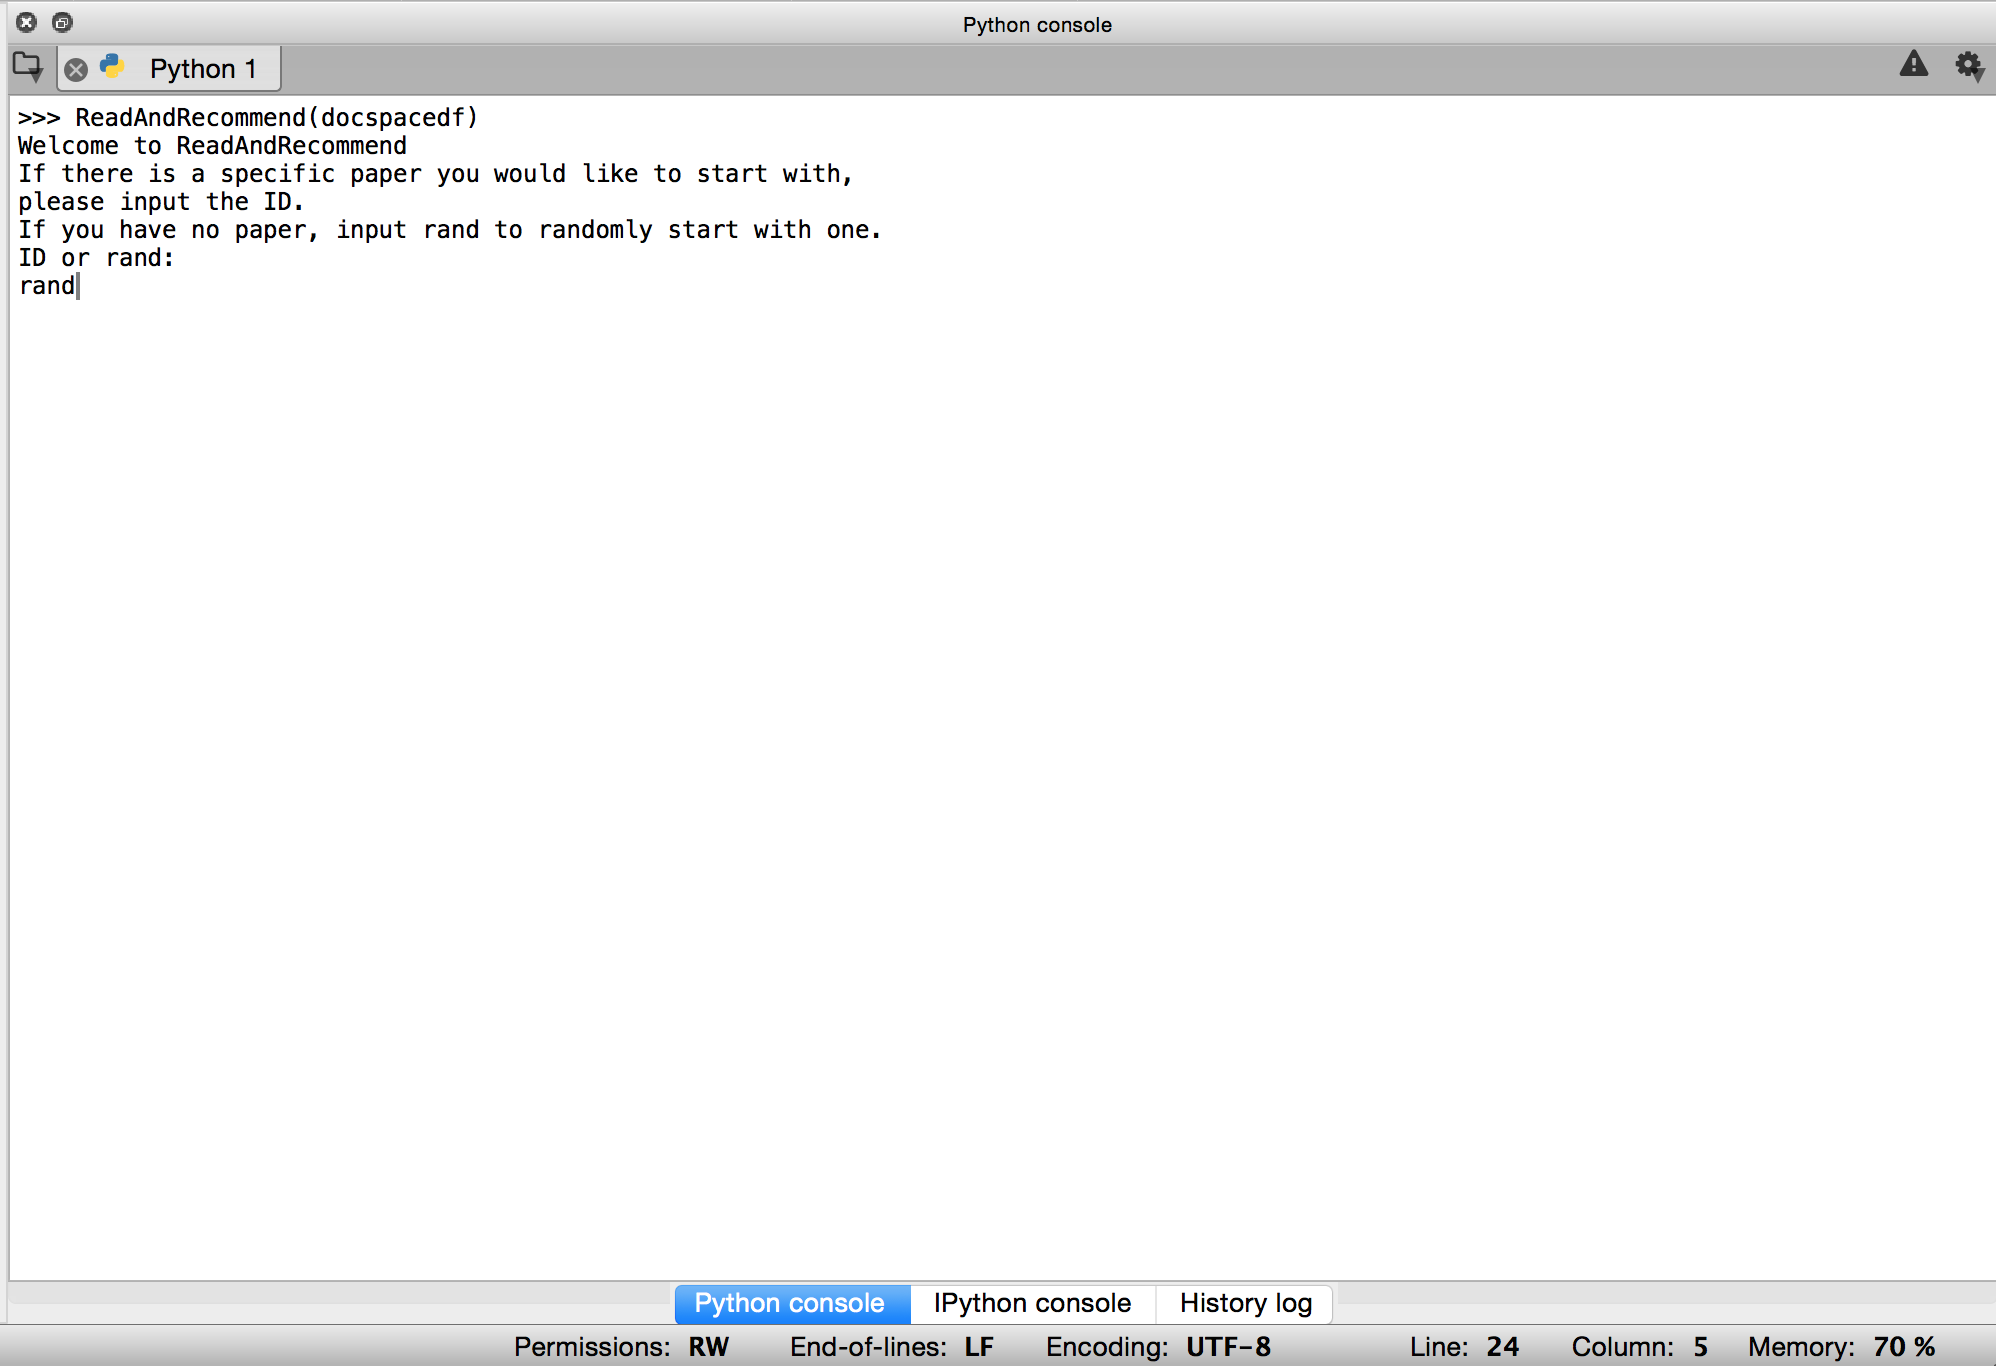
\includegraphics[scale = .35]{sshot1}

\end{center}

Running the program. Input is the $\Sigma V^t$ matrix in pandas dataframe. Columns are named by document ID. 

\begin{center}

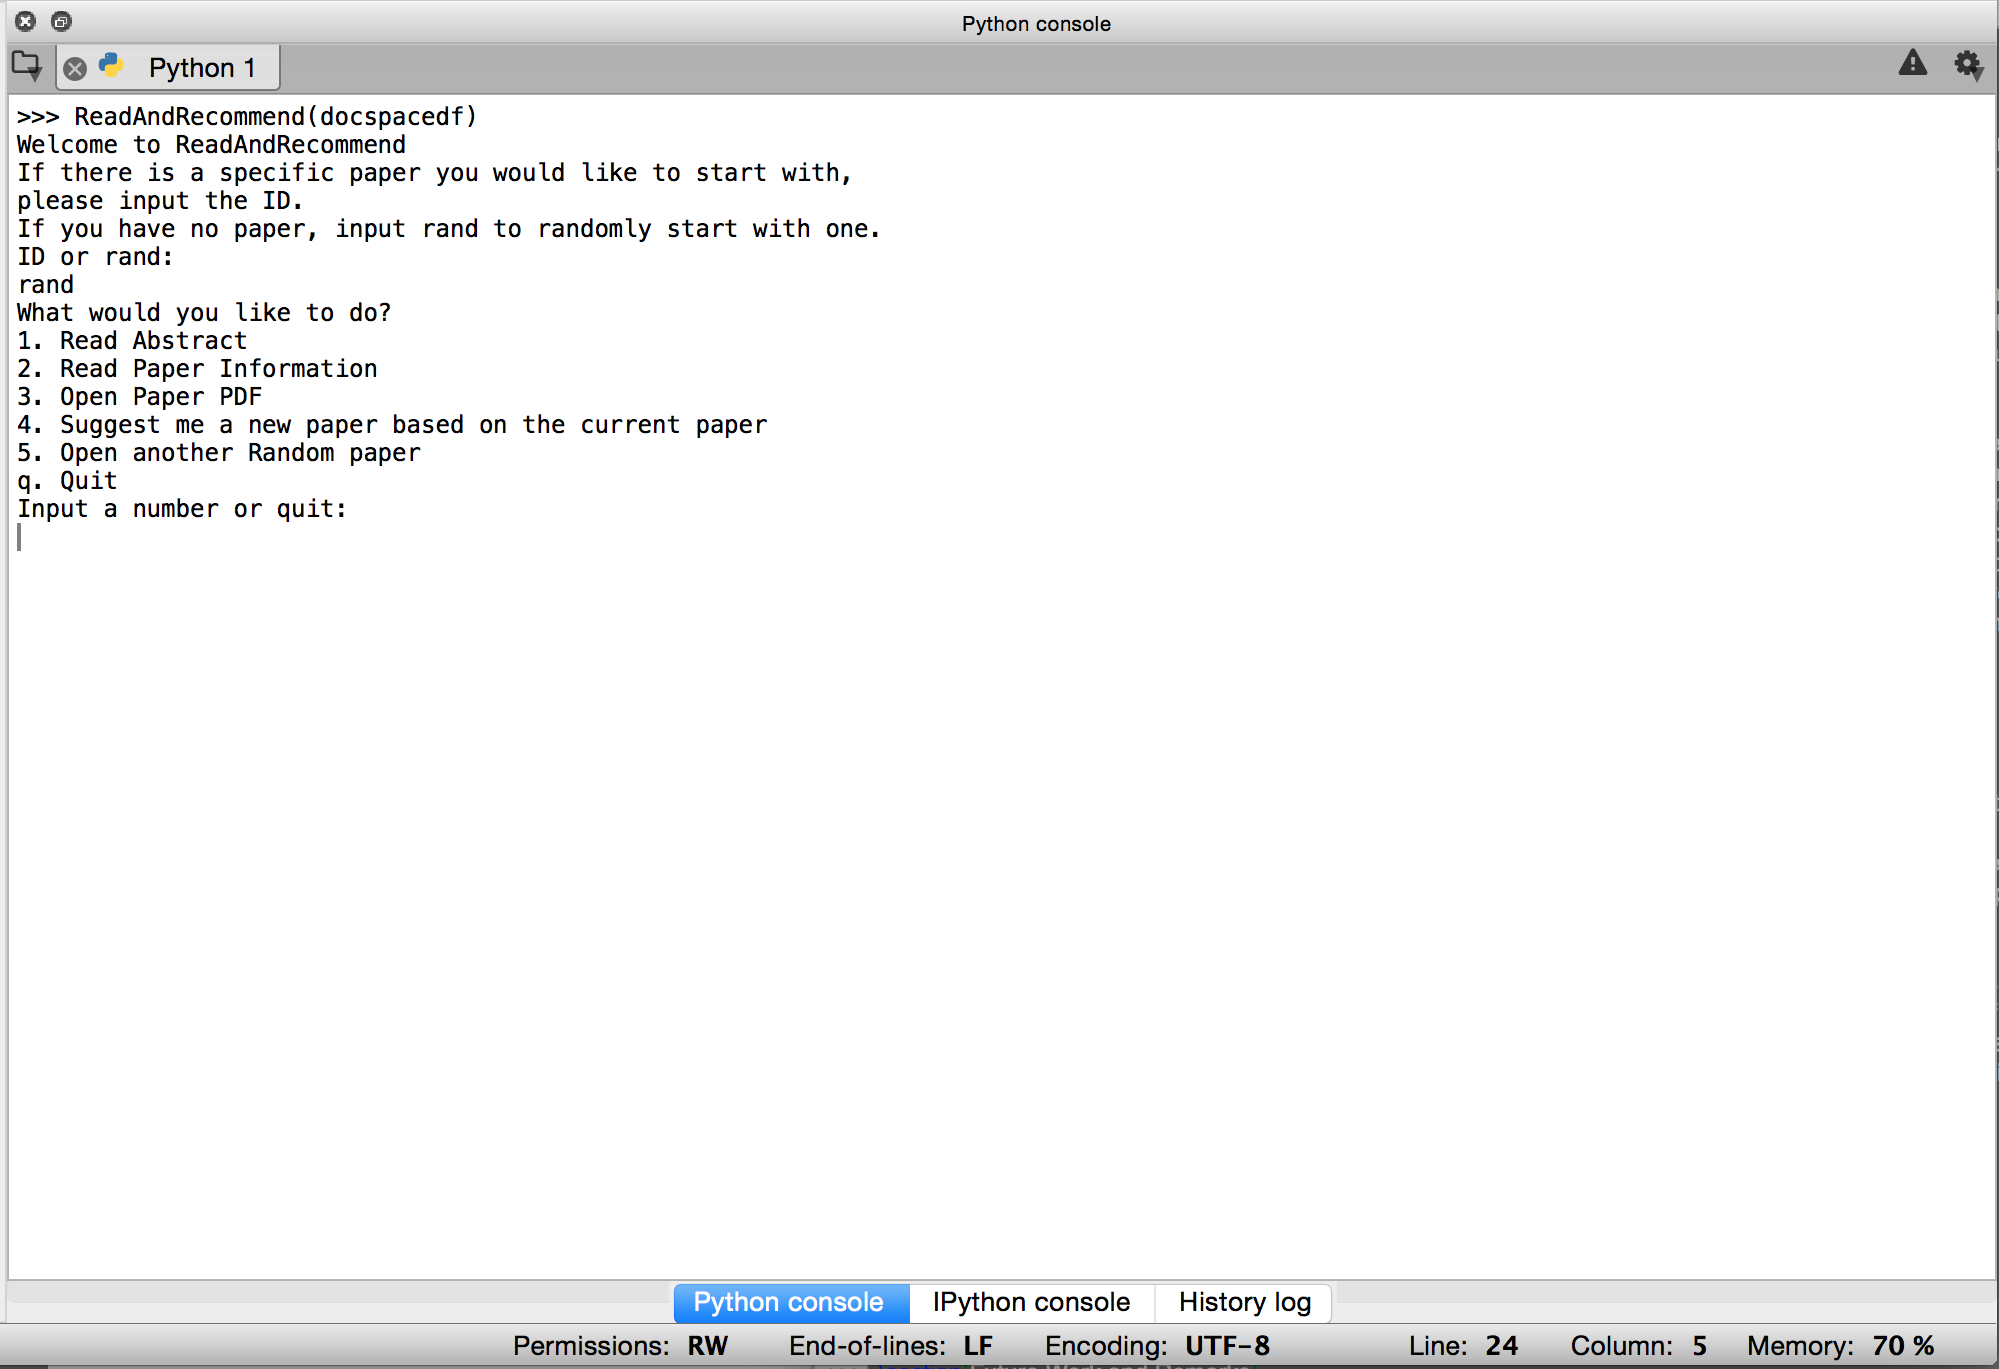
\includegraphics[scale = .35]{sshot2}

\end{center}

Once a paper has been established. This is the main loop of the code. It prompts an action from a list of selections. 

\begin{center}

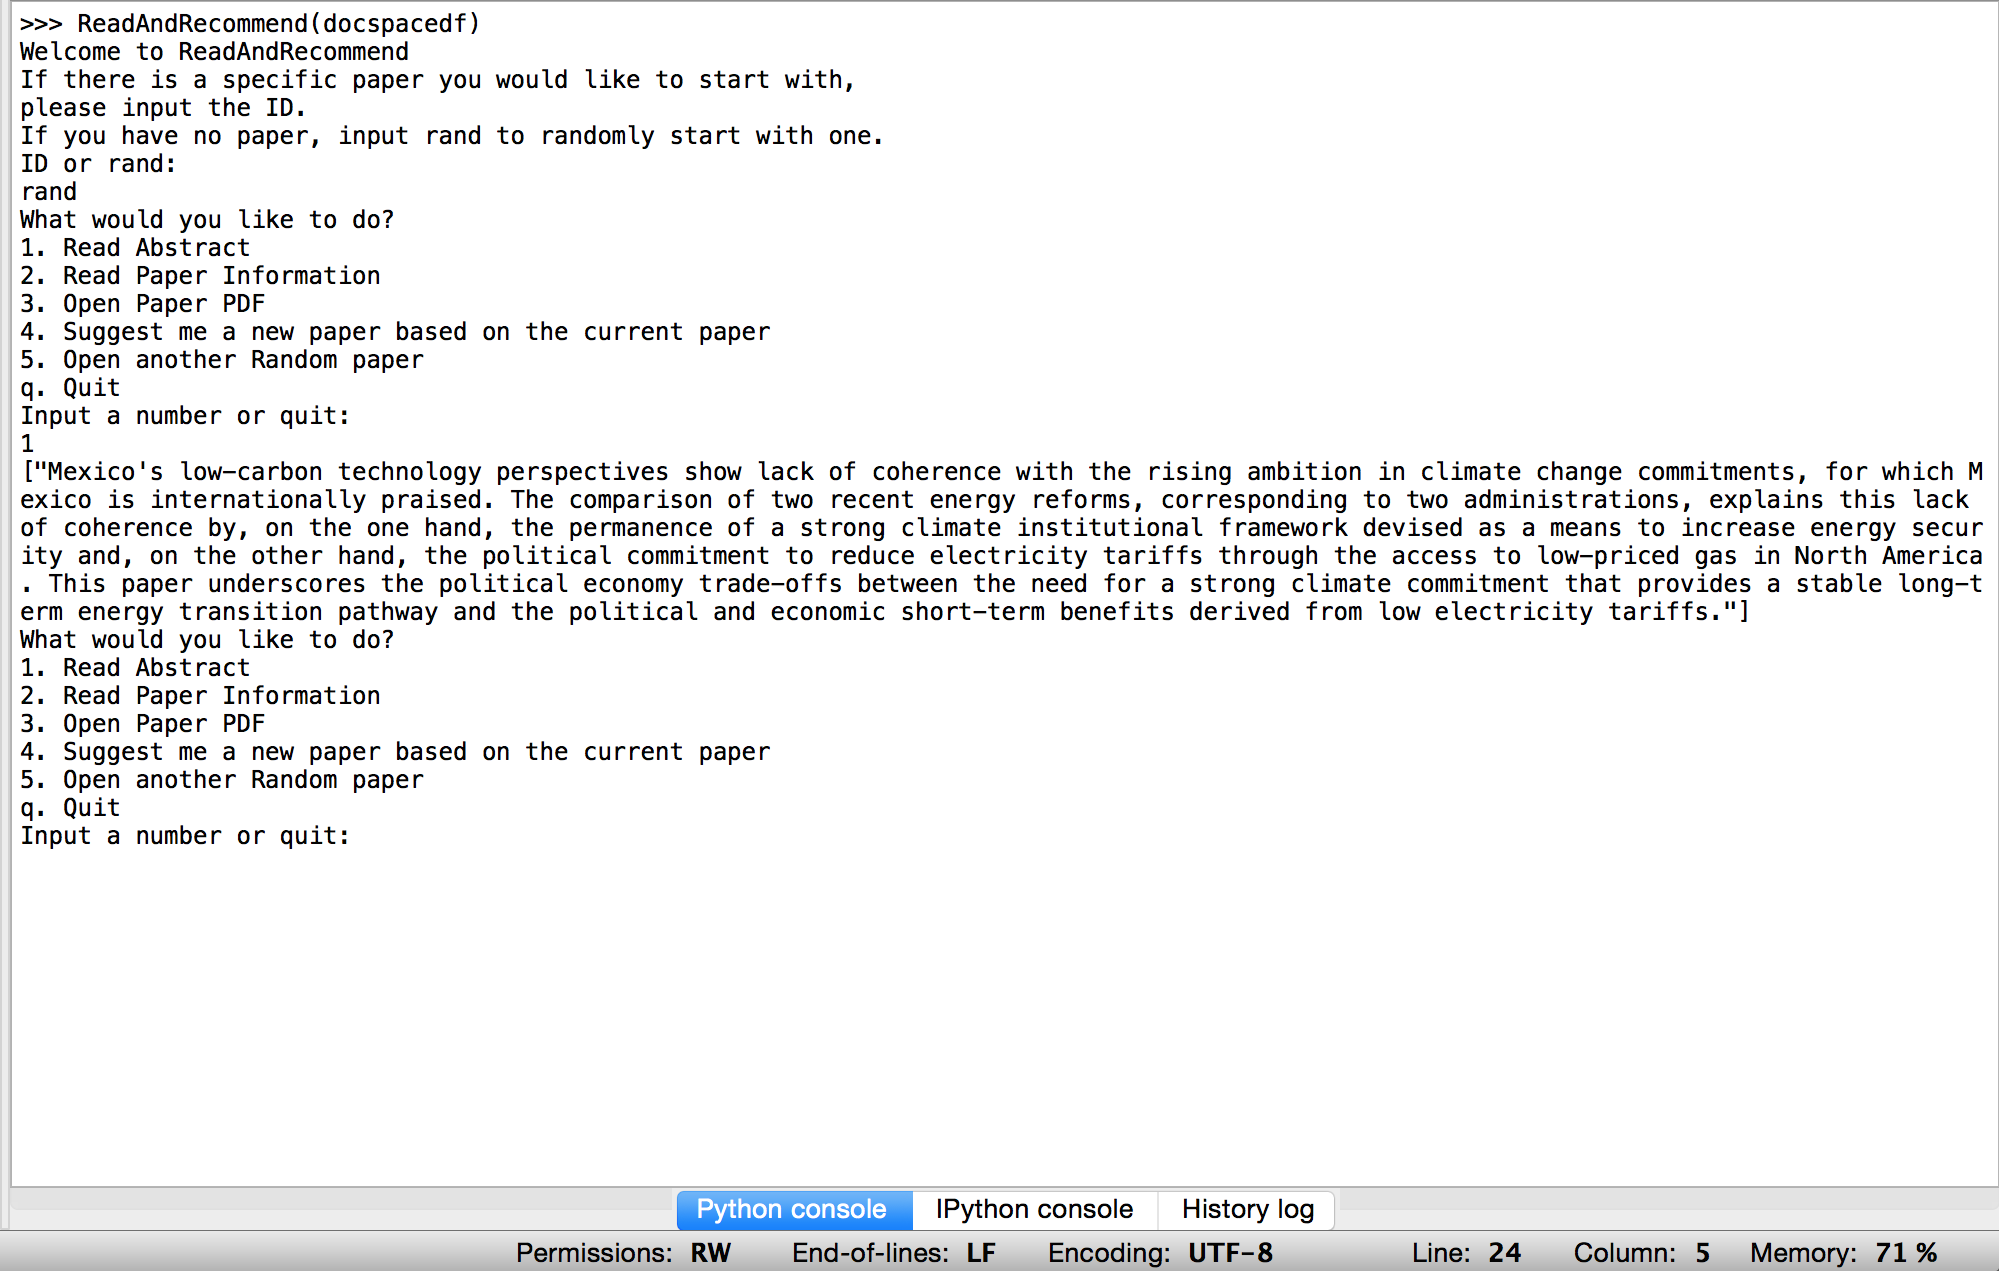
\includegraphics[scale = .35]{sshot3}

\end{center}

Option 1 produces the abstract of the current paper. It does this by pulling the abstract from the metadata. Not all metadata files contain the abstacts, therefore the code will occasionally except and print an error instead. 

\begin{center}

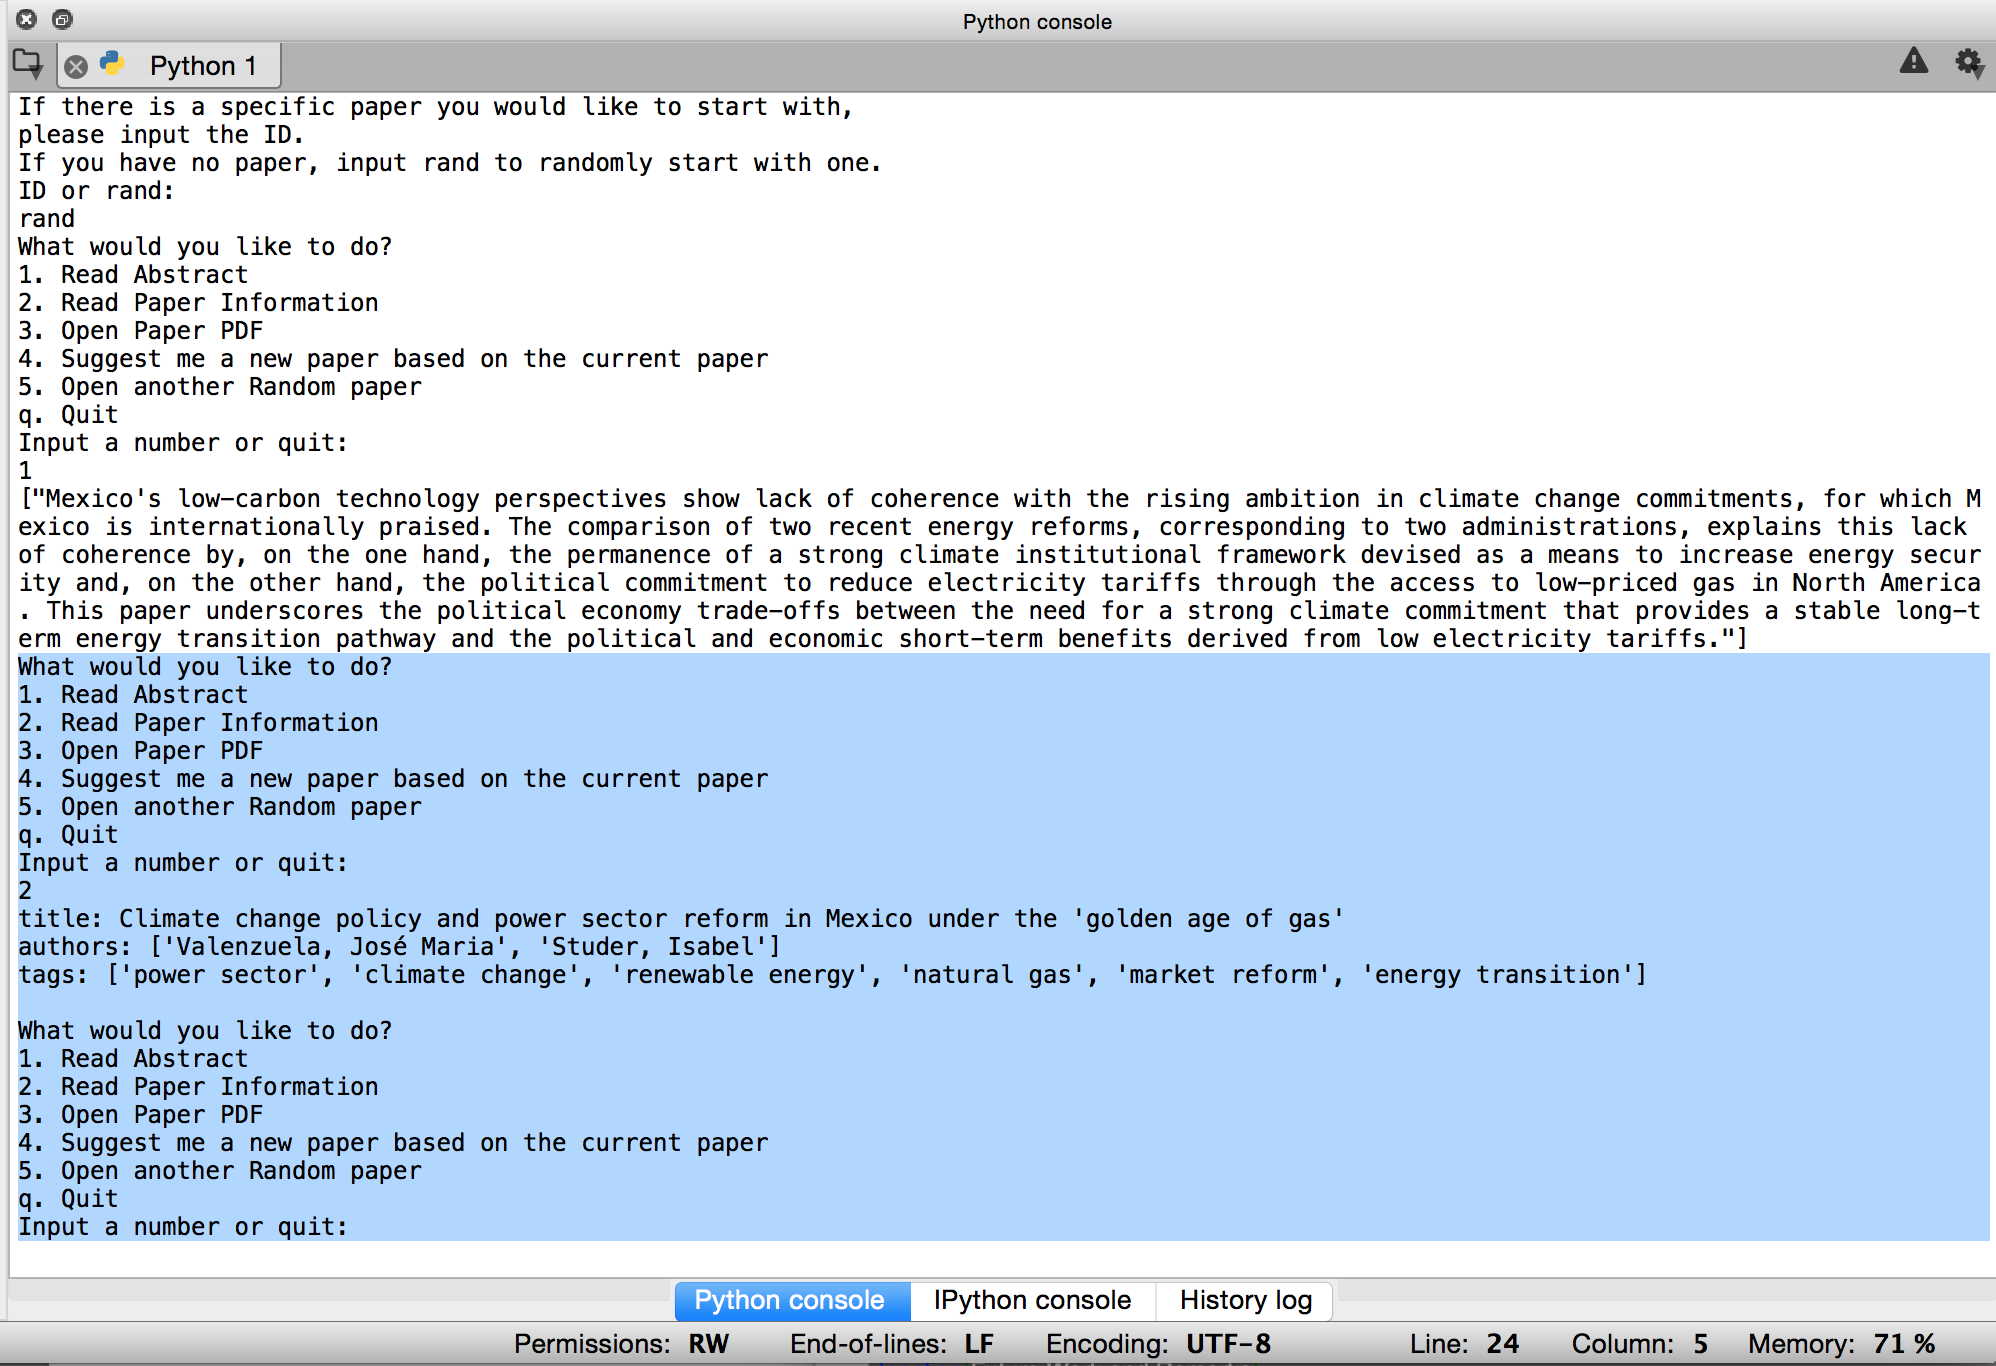
\includegraphics[scale = .35]{sshot4}

\end{center}

Option 2 produces the title, authors, and tags associated with the current paper. Occasionally, the metadata will not have the subject tags, and the code will except and print an error. 

\begin{center}

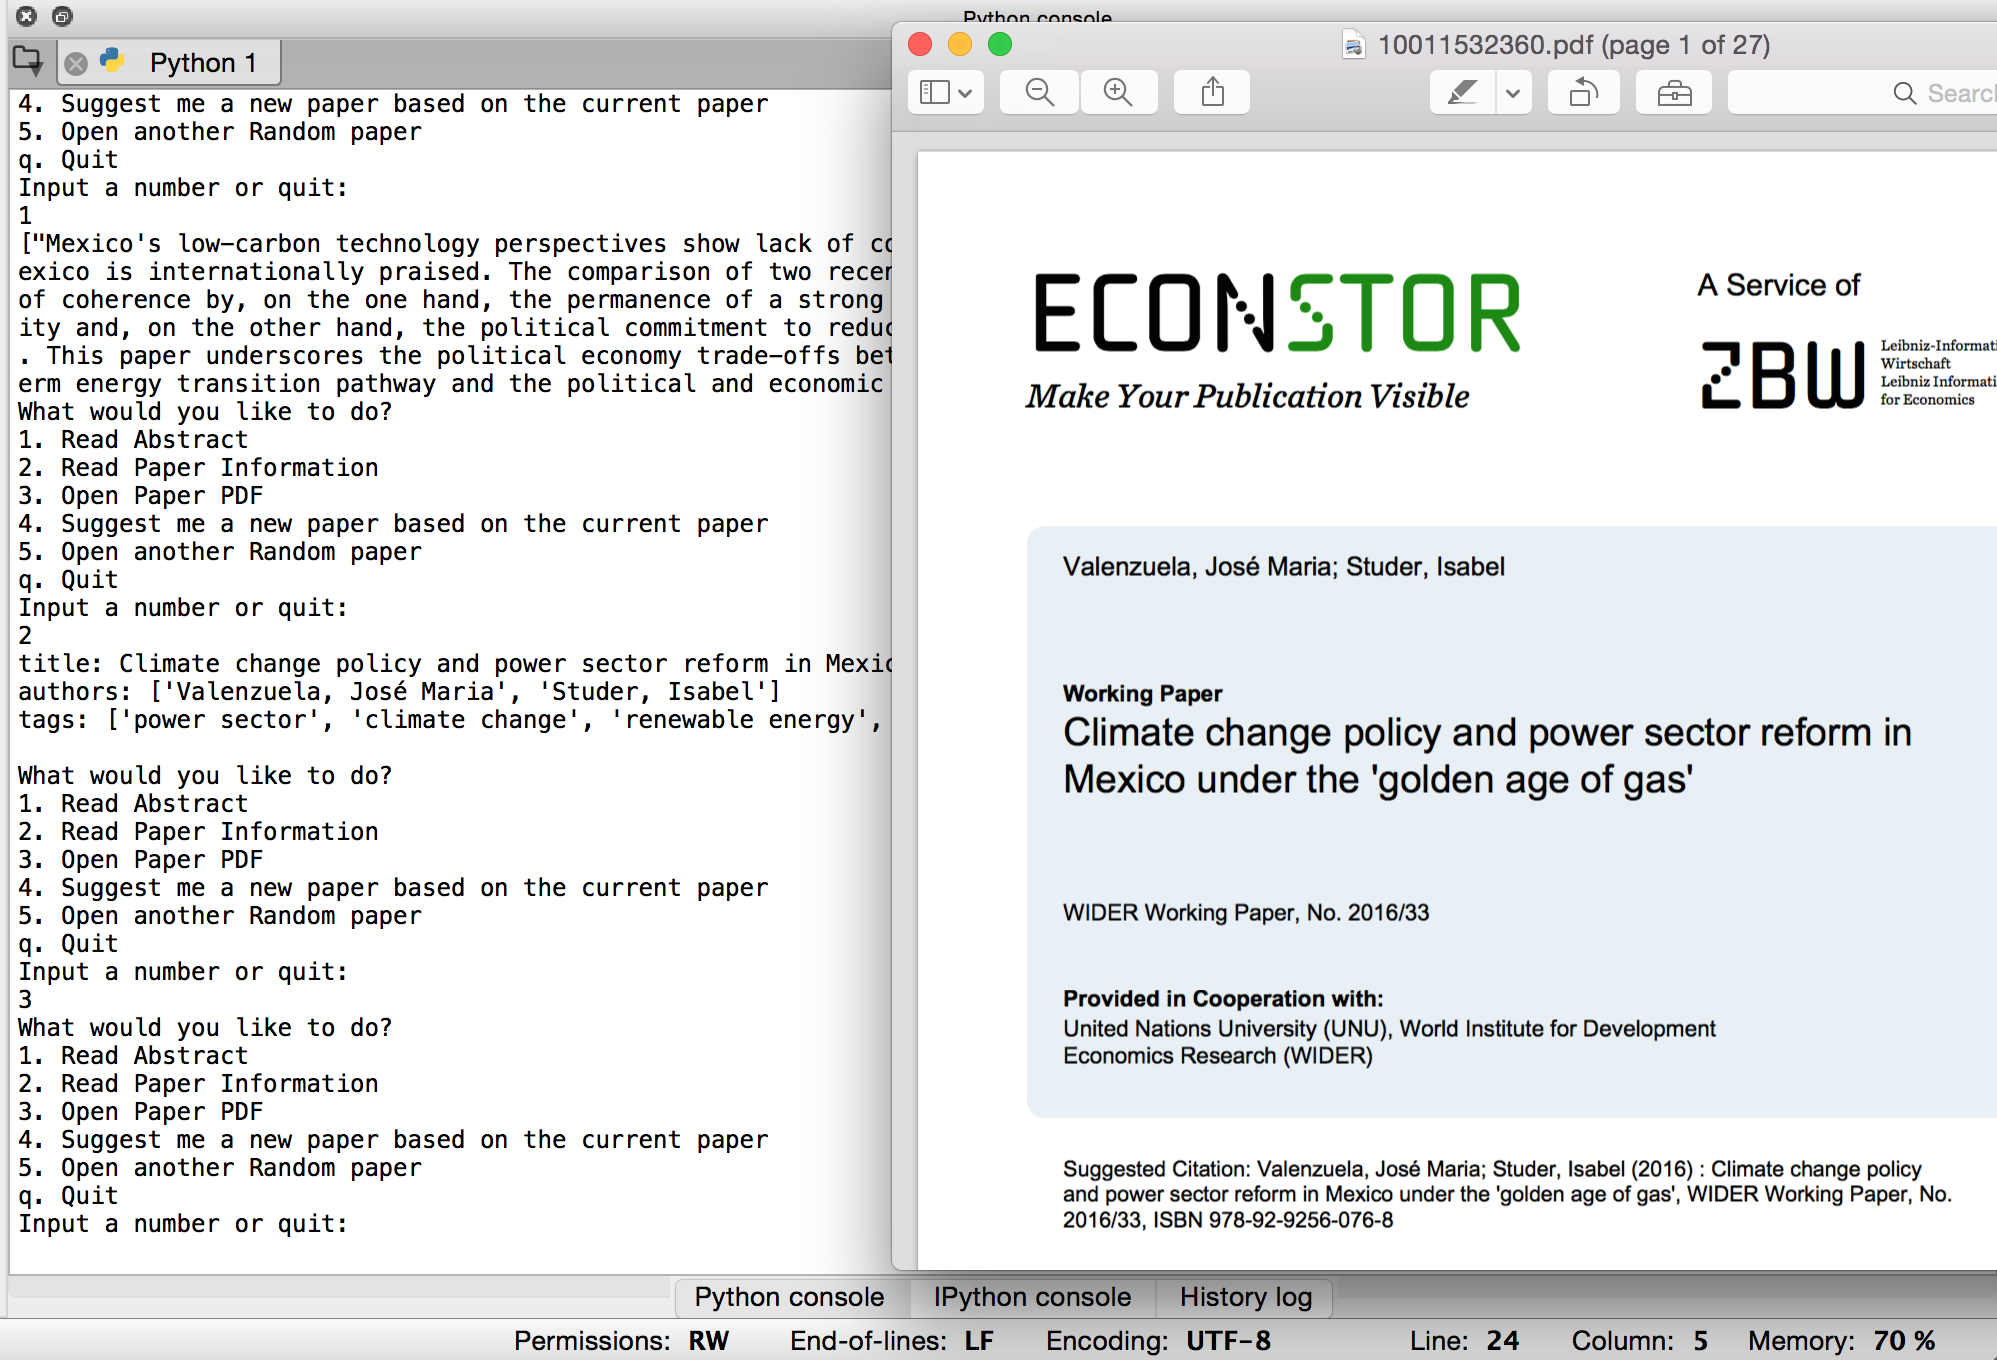
\includegraphics[scale = .35]{sshot5}

\end{center}

Option 3 will open the PDF with whatever is the default application on the current machine for handling PDFs.
 
 \begin{center}
 
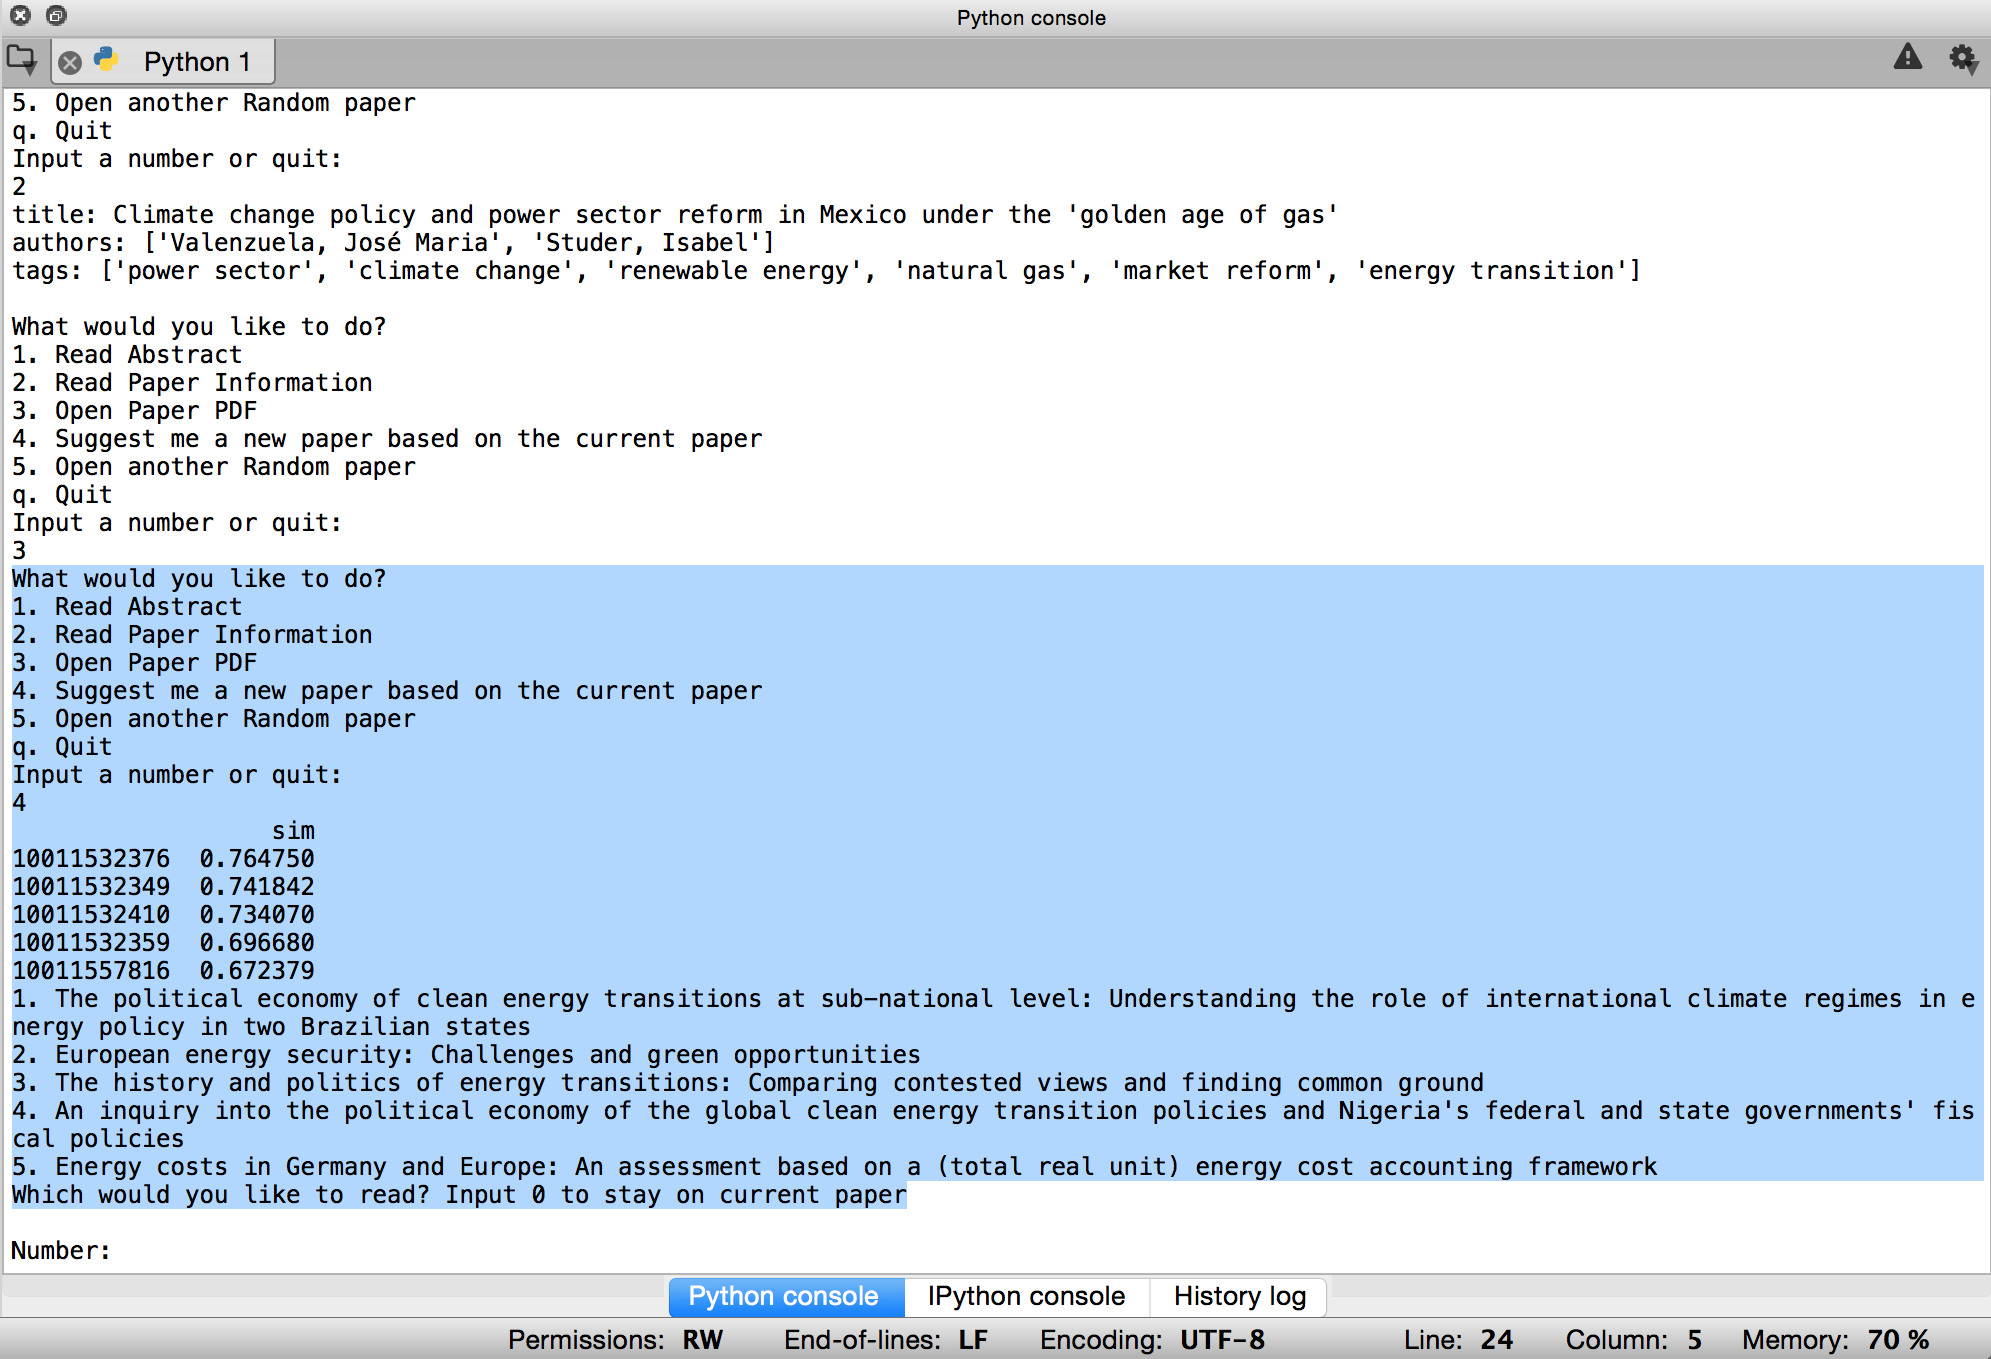
\includegraphics[scale = .35]{sshot6}

\end{center}

Option 4 calls the CosineSim function to find the lowest similarity measures. The printing of the ID numbers and their respective similarities are from the CosineSim function itself and not ReadAndRecommend. The IDs' titles are called so that the user may make a decision about what paper to read next. 

\section{Analysis} 

Although only a comprehensive function was designed for EconBiz, the CosineSimilarity function that comprises the most important part of the project was tested on both datasets for performance analysis. Since the ultimate goal however is to make good suggestions from a subjective human perspective, it is not feasible to produce any meaningful metrics for success without having a significant user base to gather feedback from. However, we will report our basic findings and remarks on the process. 

The suggestion by cosine similarity produced incredibly useful results for the arXiv hep-ph data set. Suggestions for papers were almost within the same specific topic nearly all the time. For example, a paper on a specific point of chiral perturbation theory only produced suggestions that were heavily within chiral perturbation theory. The top 5 suggestions were in fact so good that the code originally did not even print the similarity measures, since of how unnecessary they are. 

For the EconBiz dataset, results were far more mixed. Suggestions that had cosine similarity of at least .80 demonstrated similar performances seen in the arXiv data set. However, it seemed to have very little consistency in suggestion for measures less than .65 with some suggestions tangentially related and others that weren't relevant at all. 

However, this is not unexpected. The arXiv dataset was 3000 papers solely in a single specific topic within the field of physics while the EconBiz was 7000 papers across all of economics. Essentially the samples greatly differ in the 'density' relative to the size of the subject the sample is suppose to cover. We estimate that the arXiv dataset is probably at least 50 times more dense (by virtue of how large high energy physics is compared to all of physics). If our EconBiz dataset was sufficiently large, we expect that its performance would be equally impressive as the arXiv hep-ph set.

\section{Future Work}

Obviously, one of the shortcomings of this paper is relatively small size of the corpus. The sample we used is not large enough to confidently justify our findings as a proof of concept for implementation of SVD to actual literature hosting sites. Because our sample is unrepresentative of the scale of the problem that hosting sites face, we have relatively avoided the computational complexity issues that might arise. 

Notably, SVD produces scalability issues as the number of papers increase. Although a literature hosting site would have more computation resources at their disposal, the cubic computational complexity guarantees that the time required for SVD will grow extremely quickly as the database grows. However as shown by the arXiv dataset, there is a distinct advantage in segregating a field's literature into specific topics when it comes to suggestion of relevant papers, so there may be practical answers to the size of the corpus by splitting the corpus. This results in more of an organizational question on the side of database implementation by the hosting sites. 

This paper has also ignored the issue of a dynamically changing database of papers. That is, how do we update the SVD in an efficient manner to accommodate for new documents (and possibly new terms) being added to the corpus? SVD on an extremely large corpus will take a great deal of computation, and it is infeasible to rerun a whole new SVD very often. This question will be one of the most important to solve before being able to advocate use of SVD for actual literature recommendation. 

Lastly, one of the tasks that was originally planned to be tackled in this paper was using Bayesian filtering to determine the "reading preferences" of the users. We had planned to model the density of papers read by a user in the Feature vs. Document space. At that point, one can suggest effectively by just matching spatially within the Feature vs. Document. 

\begin{thebibliography}{9}



\bibitem{GeneralRef} 
Bannerjee, Sudipto and  Anindya, Roy (2014).
\textit{Linear Algebra and Matrix Analysis for Statistics}. Chapman and Hall/CRC Texts in Statistical Science.

\bibitem{SVDcomp}
Cline, Alan and Dhillon, Inderjit (2013).  Computation of the Singular Value Decomposition. Chapter 45 of \textit{Handbook of Linear Algebra 2nd ed}. Chapman and Hall/CRC Texts in Statistical Science. Retrieved from \textit{http://www.cs.utexas.edu/users/inderjit/public\_papers/HLA\_SVD.pdf}

\bibitem{LSAprocess}
Landauer, Thomas and Dumais, Susan (2008). Latent Semantic Analysis. Scholarpedia.
Retrieved from

\textit{http://www.scholarpedia.org/article/Latent\_semantic\_analysis}

 \bibitem{LSA} 
Wiemer-Hastings, Peter (2004). Latent Semantic Analysis. Retrieved from \textit{http://reed.cs.depaul.edu/peterh/papers/Wiemer-HastingsEnc-LSA.pdf}



\end{thebibliography} 
 


\end{document}